%%%%%%%%%%%%%%%%%%%%%%%%%%%%%%%%%%%%%%%%%%%%%%%%%%%%%%%%%%%%%%%%%%%%%%
% How to use writeLaTeX: 
%
% You edit the source code here on the left, and the preview on the
% right shows you the result within a few seconds.
%
% Bookmark this page and share the URL with your co-authors. They can
% edit at the same time!
%
% You can upload figures, bibliographies, custom classes and
% styles using the files menu.
%
%%%%%%%%%%%%%%%%%%%%%%%%%%%%%%%%%%%%%%%%%%%%%%%%%%%%%%%%%%%%%%%%%%%%%%

\documentclass[12pt]{article}

\usepackage{sbc-template}

\usepackage{graphicx,url}

%\usepackage[brazil]{babel}   
\usepackage[utf8]{inputenc}  

\usepackage{amsmath}

     
\sloppy

\title{Ensaio Sobre Falácias Lógicas\\ Em Debates Políticos}

\author{Enzo H. Andrade\inst{1}, Gian Lucca D. Paneto\inst{2}, Heitor L. Peixoto
\inst{3}}


\address{Instituto Federal do Espírito Santo (Ifes)\\Campus Serra}

\begin{document} 

\maketitle


\begin{resumo} 
  Este artigo investiga a presença e o efeito das falácias lógicas em debates políticos, evidenciando como tais falácias distorcem a razão do pensamento lógico e, portanto, influenciam a realidade e, consequentemente – a consciência, percepção pública e até mesmo a escolha eleitoral. Com uma abordagem qualitativa, este estudo analisa transcrições de debates políticos em vários períodos e contextos, identificando falácias mais frequentes, a exemplo de ataques pessoais, apelos emocionais e falsas dicotomias, dentre outros. Observa-se que, por meio dessas falácias, a realidade é intencionalmente manipulada com o objetivo de desfocar-se de assuntos pertinentes, espalhando desinformação e polarizando o discurso. Por fim, este trabalho discute o papel da tecnologia nesse processo, notando-se como redes sociais e plataformas digitais facilitam a disseminação mais rápida de tais alegações falaciosas, arruinando a ética do público engajado. Conclui-se com a sugestão de um entendimento crítico e desenvolvimento do conhecimento sobre tais discursos lembrados não só para os eleitores, mas para qualquer pessoa politicamente engajada.
\end{resumo}


\section{Introdução}
\subsection{Contexto}
Os debates políticos possuem papel de destaque na manutenção do perfil democrático social. A exposição de diversas correntes de pensamento em uma única discussão é uma forma eficaz de esclarecer opiniões e desenvolver o senso crítico. Dessa forma, o debate político busca perpetuar a transparência e a responsabilidade em relação às opiniões expostas. Entretanto, a presença de falácias lógicas — artifícios argumentativos que invalidam o raciocínio lógico — \cite{Domina:1} pode comprometer essa função, visando mais à persuasão do que à busca pela verdade. 

Os debates políticos remontam tempos antigos, como na Grécia Antiga, na democracia ateniense. Com isso, surge-se o interesse de analisar a argumentação e raciocínios, essa prática é chamada de teoria da argumentação, com origens em lógica, dialética e retórica. Autores clássicos como Aristóteles e Cícero, têm relevância direta nessa problemática atual, pois eles fundamentam nossas definições de falácias lógicas.

O termo falácia deriva do verbo latino \textit{fallere}, que significa enganar. Designa-se por falácia um argumento de raciocínio errado com aparência de verdadeiro. Na lógica e na retórica, uma falácia é um argumento logicamente incoerente, sem fundamento, inválido ou falho na tentativa de provar eficazmente o que alega \cite{Wikipédia-2}. Além disso, Hamad (2022) introduz o conceito de "regras de razoabilidade" as quais são rompidas pelo uso de falácias \cite{Hamad-3}. Tal argumento é empregado nos discursos para dissolver a diferença de pensamentos de modo a aceitar o ponto de vista apelando à razoabilidade da outra parte, persuadindo assim os ouvintes com o ponto de vista do orador \cite{Zilin-4}. Portanto, as falácias se tornam um efetivo instrumento de manipulação e controle através do discurso.

Entretanto, alguns autores concordam com o uso de falácias e entendem como ferramente inerente
a existência de um discurso político. Imani (2021) afirma que o objetivo principal do discurso político é persuadir as pessoas, esse propósito não pode ser alcançado a menos que o público veja o mundo de acordo com os desejos dos políticos. Na verdade, o discurso político pretende impor certas crenças e atitudes às pessoas, essas crenças e atitudes compreendem as ideologias subjacentes dos políticos e, de acordo com essas ideologias, os políticos constroem sua linguagem pela qual visam persuadir as pessoas e, assim, exercer poder e domínio sobre elas (Van Dijk, 2006). Assim, é valido considerar a natureza de um debate político e as consequências de usos desses instrumentos argumentativos.

Com a redemocratização e as eleições civis diretas no Brasil em 1989, os debates presidenciais passaram a ser televisionados ao-vivo, e, desde então, toda eleição presidencial possuiu debates (exceto 1998, onde o então presidente Fernando Henrique Cardoso se negou a participar de debates). Em julho de 2000, em pesquisa realizada pelo Datafolha \cite{Datafolha-11}, os entrevistados caracterizaram em maioria o debate política como "muito importante para decidir o seu voto".

Dada a importância do debate na escolha do chefe de Estado no Brasil, é crucial ter exatidão nas falas, visto que novas tecnologias que surgiram nas últimas décadas como "Fake News" e "Deep Fakes" possibilitando a manipulação de informação e portanto podem resultar no aumento de argumentos falaciosos, os quais podem interferir negativamente no destino do país.

A relevância desta pesquisa está na análise da frequência e evolução das falácias em debates políticos presidenciais no Brasil entre 1989 e 2022, permitindo compreender como esses artifícios podem influenciar a tomada de decisões em cenários nacionais, e como a inovação e tecnologias de "fact-checking" e gravações podem ter interferido na prevalência de falácias. Assim, a problemática abordada se concentra na prevalência das falácias lógicas e nos efeitos da falta de consciência crítica sobre esses instrumentos argumentativos.

\section{Referencial Teórico} \label{sec:Referencial Teorico}
A análise dos debates políticos foi realizada tendo como referência a literatura que trata de conceitos de falácias lógicas e seus respectivos usos em frases. A literatura que aponta a construção de argumentos falaciosos e como construir argumentos válidos tem como ponto central a reflexão sobre a natureza do discurso e dos usos das falácias e a existência de situações que torne "necessário" o uso desses artifícios manipulatórios. necessidade de múltiplos atores e visões para conseguir abarcar a complexidade do conhecimento no estágio atual do desenvolvimento científico e tecnológico (Christopher, 2007; Van Dijk, 2006; AL-Rikabi, 2022). Além disso, no caso específico do uso de falácias em debates políticos, pesquisas e artigos científicos publicados foram usados como referência na análise dos debates (Hamad(2022), Zilin(2018)).Entretanto, é notório a inexistência ou, ao menos, falta de notoriedade de artigos e pesquisas que abordem o cenário nacional. Em consonância com as recentes inovações da tecnologia e de geração de texto, a analise e estudo foram auxiliados com IAs além de códigos em Python.

Desse modo, a os debates discutidos nesse ensaio referenciam, em sua maioria, o primeiro turno de todos os anos, exceto alguns anos em que não foi possível achar um vídeo de primeiro turno e, portanto, foi substituído pelo debate do 2° Turno. De mesmo modo, em uma tentativa de evitar desvios de dados, foi padronizado o uso de debates da emissora Band em todos os casos que foram possíveis.

Nos exercícios literários submetidos a análise incorporaram a identificação de falácias mais comuns conforme descrito em pesquisas anteriores. Baseado em pesquisas de Hamad (2022) em que foram expostas 10 discursos no cenário político americano, ele chegou no resultado de que as falácias mais recorrentes são: "Ad hominem", "A pathetic fallacy (pathos)" e "Magnifying what has 
been left unexpressed".

Além disso, compreendendo a diferença de pensamento na literatura que aborda as falácias lógicas, esse ensaio tem por conduta a analise dos dados sobre o assunto e a exposição de contextos de época que podem ter gerado alguma alteração no discurso, além de evidenciar os possíveis malefícios de discursos falaciosos no cenário politico brasileiro. Assim, entrevista e reportagens de época foram analisadas para compor o estudo de contexto do período de discussão (Datafolha, G1, Infomoney, Globo).

Portanto, esse ensaio reúne aspectos de conhecimento codificado de materiais acadêmicos na análise e implementação da lógica em frases e citações mas, também, considera o conhecimento situacional da frase em questão para possíveis discussões sobre o uso da falácia. Dessa maneira, engloba ambas as facetas necessárias na abordagem do temido dilema politico de mentiras, verdades e contradições.

\section{Discussão}

Em 1989, na primeira eleição presidencial direta após 29 anos de eleições indiretas, foi televisionado o primeiro debate do primeiro turno entre os presidenciáveis na Rede Bandeirantes. Não era apenas o primeiro debate televisionado pós-redemocratização, mas sim o primeiro debate televisionado na história do Brasil.  \cite{Band-5} 

O encontro promovido pela Band teve apresentação de Marília Gabriela e reuniu nove dos vinte e dois candidatos da disputa. Com regras mais flexíveis que as de hoje, participaram naquela ocasião os candidatos Luiz Inácio Lula da Silva (PT), Leonel Brizola (PDT), Paulo Maluf (PDS), Roberto Freire (PCB), Affonso Camargo (PTB), Aureliano Chaves (PFL), Ronaldo Caiado (PSD), Mário Covas (PSDB) e Guilherme Afif Domingos (PL). Fernando Collor (PRN) e Ulysses Guimarães (PMDB) foram convidados, mas não compareceram. No debate, assuntos como reforma agrária e a ditadura militar foram muito abordados. 

O debate foi bastante acalorado, e, com isso, um dos mais falaciosos da história. Frases como "filhotes da ditadura", de Leonel Brizola contra Paulo Maluf ficaram enraizadas no imaginário politico brasileiro. \cite{Maluf-6} Interrupções foram frequentes, juntamente com argumentos \textit{Ad Hominem}, onde candidatos atacavam pessoalmente outros candidatos. No debate politico o candidato Luís Inácio Lula da Silva disse a frase: 

"[...] a verticalização, que tornou praticamente a seleção as alianças a uma promiscuidade [...]" 

Nesta frase, o candidato afirma que a verticalização levou inevitavelmente à promiscuidade nas alianças e, portanto, se trata de uma falacia de generalização apressada afinal, não se pode concluir como o fator decisivo sem embasamento prévio e contextualizado. Usando ferramentas da lógica de predicados:

\textbf{Predicados:}
\begin{itemize}
    \item $V(x)$: $x$ é um sistema de verticalização.
    \item $P(x)$: $x$ resultou em promiscuidade.
    \item $A(x)$: $x$ resultou em seleção de alianças.
\end{itemize}

\textbf{Expressão lógica:}

\[
\forall x \, (V(x) \rightarrow (A(x) \land P(x)))
\]

Desse modo, no contexto dessa frase, indica que o sistema de verticalização resulta em ambas consequências.

Manipulações, mentiras e falácias foram muito usadas durante toda campanha de 1989. No programa "Eleições 89", por exemplo, exibido pela Globo em 03/12/89, Collor foi agraciado com um tempo de 22 minutos e 2 segundos, enquanto Lula não recebeu nenhum tempo. \cite{Theodoro-7}


\begin{table}[ht]
\centering
\caption{Dados das Avaliações do Debate de 1989}
\label{tab:exTable1}
\begin{tabular}{l r}
\hline
\textbf{Variável} & \textbf{Valor} \\
\hline
Total de frases & 249 \\
Total de falácias & 38 \\
Média de falácias por frase & 0,1526104418 \\
\hline
\end{tabular}
\end{table}

A partir dessa tabela, podemos inferir relações entre o total de frases (notoriamente mais usadas por Collor) e o total de falácias, o que demonstra, ao menos estatisticamente, o poder que um maior uso de falácias tem no processo de manipulação e convencimento com o argumento. A eleição terminaria com Collor vencedor e posteriormente destituído do cargo em 1992. Ele renunciou à presidência em 29 de dezembro, pouco antes de ser formalmente afastado pelo Senado no processo de impeachment. O seu vice presidente assumiria, Itamar Franco. Na época, o mandato presidencial durava 5 anos e não dava a opção de reeleição. Portanto, uma nova eleição e um novo debate só aconteceria em 1994.

As eleições presidenciais de 1994 no Brasil ocorreram em um contexto de grande mudança econômica e política. O país estava saindo de um período de hiperinflação e instabilidade econômica. O Plano Real, implementado no início de 1994, conseguiu estabilizar a economia e reduzir drasticamente a inflação, o que teve um impacto significativo no cenário eleitoral.

O sociólogo e escritor Fernando Henrique Cardoso foi nomeado por Itamar Franco para ser Ministro da Fazenda, e chefiou a implementação do Plano Real, e era bastante popular. Fernando Henrique acabaria sendo o primeiro e único presidente eleito no Brasil em primeiro turno.

O primeiro debate foi, novamente, televisionado pela Rede Bandeirantes. Participaram do debate Fernando Henrique Cardoso (PSDB), Luiz Inácio Lula da Silva (PT), Orestes Quércia (PMDB), Leonel Brizola (PDT), Hernani Goulart Fortuna (PSC), Esperidião Amin (PPR) e Enéas Carneiro (PRONA). O debate, novamente foi mediado por Marília Gabriela. 

O grande assunto era a hiperinflação que havia há pouco sido arrefecida, reformas sociais e a corrupção. O debate foi repleto de falácias, espantalhos, Ad Hominem, e falácias apelativas à emoção. 

\begin{table}[ht]
\centering
\caption{Dados das Avaliações do Debate de 1994}
\label{tab:exTable1}
\begin{tabular}{l r}
\hline
\textbf{Variável} & \textbf{Valor} \\
\hline
Total de frases & 554 \\
Total de falácias & 96 \\
Média de falácias por frase & 0,1732851986 \\
\hline
\end{tabular}
\end{table}

Em 1998, não houve qualquer debate. Fernando Henrique Cardoso preferiu se ausentar de todos os convites, muito provavelmente por ser amplamente popular e por fraqueza da oposição. Fernando acabaria sendo reeleito em primeiro turno com 53,6\% dos votos \cite{MemoriaGlobo-8}.

O primeiro debate de 2002 foi, tradicionalmente, realizado pela Bandeirantes. Participaram do debate Luiz Inácio Lula da Silva (PT), José Serra (PSDB), Ciro Gomes (PPS) e Anthony Garotinho (PSB). O debate contou com regras mais rígidas e um notável respeito ao momento de fala de fala de outros candidatos, se comparado com os debates anteriores. Apesar disto, o debate teve alto nível de falácias. Portanto, a moderação no tom de voz e nas interrupções não são garantia de argumentos bem construídos. A exemplo, o candidato garotinho nesse debate disse a frase:

"[...] as elites brasileiras se conformaram durante muito tempo em fazer o jogo de subserviência."


\begin{table}[ht]
\centering
\caption{Dados das Avaliações do Debate de 2002}
\label{tab:exTable1}
\begin{tabular}{l r}
\hline
\textbf{Variável} & \textbf{Valor} \\
\hline
Total de frases & 253 \\
Total de falácias & 39 \\
Média de falácias por frase & 0,1541501976 \\
\hline
\end{tabular}
\end{table}

Lula acabaria por ser vencedor da eleição após um segundo turno com José Serra.

Em 2006, Lula foi reeleito, mas não participou de nenhum debate no primeiro turno. Lula era líder das intenções de voto \cite{InfoMoney-12}). Coisa que também aconteceu com FHC em 1998. O debate na Bandeirantes foi mediado pela primeira vez pelo jornalista Ricardo Boechat. Participaram do debate Geraldo Alckmin (PSDB), Luciano Bivar (PSL), Cristovam Buarque (PDT), José Maria Eymael (PSDC) e Heloísa Helena (PSOL). 

Boechat não teve grandes problemas para mediar o debate, foi ameno e respeitoso. Ainda, nota-se um padrão. Cada vez mais, a quantidade de falácias diminui, o padrão de diminuição nas médias podem ser vistas, tanto em 2006, quanto 2002 e 1994.

\begin{table}[ht]
\centering
\caption{Dados das Avaliações do Debate de 2006}
\label{tab:exTable1}
\begin{tabular}{l r}
\hline
\textbf{Variável} & \textbf{Valor} \\
\hline
Total de frases & 684 \\
Total de falácias & 76 \\
Média de falácias por frase & 0,1111111111 \\
\hline
\end{tabular}
\end{table}

Em 2010, novamente na Band, o debate contou com a presença dos principais candidatos: Dilma Rousseff (PT), José Serra (PSDB), Marina Silva (PV) e Plínio de Arruda Sampaio (PSOL). Dilma sairia vencedora da eleição em um segundo turno com José Serra. O debate segue com a tendência de diminuição da média. Apesar de uma oposição forte de José Serra na campanha, o debate foi calmo. Esse debate marcaria o sopé dentre todos os debates analisados nesse ensaio. 

\begin{table}[ht]
\centering
\caption{Dados das Avaliações do Debate de 2010}
\label{tab:exTable1}
\begin{tabular}{l r}
\hline
\textbf{Variável} & \textbf{Valor} \\
\hline
Total de frases & 863 \\
Total de falácias & 76 \\
Média de falácias por frase & 0,08806488992 \\
\hline
\end{tabular}
\end{table}

O contexto político do Brasil em 2014 foi marcado por um cenário de intensas disputas eleitorais e crescente polarização. O país se encontrava em um momento de transição, onde a reeleição da então presidente Dilma Rousseff (PT) era vista como um reflexo de um período de mudanças significativas que se iniciaram com a presidência de Luiz Inácio Lula da Silva. Contudo, o crescimento da polarização política começou a se intensificar, em grande parte, devido a uma série de fatores econômicos e sociais.

Os indicadores sociais estáveis na era Lula já não eram os mesmos com Dilma \cite{IBRE-9}. A oposição crescia cada vez mais, e era cada vez mais ferrenha. Contextos como os protestos de junho de 2013 e os escândalos de corrupção na Copa do Mundo de 2014 ajudaram ainda mais na polarização. 

A ascensão do conservadorismo nas mídias sociais foram muito relevantes para adesão as manifestações \cite{Esther-10}, movimentos como o “não vai ter Copa” e “fora Dilma” que começaram nas redes sociais foram muito importantes na criação de um candidato da oposição forte que se opunha ao petismo, Aécio Neves.

Todo esse contexto se liga diretamente com o debate político de 2014, onde vemos as consequências do da polarização política no Brasil. Na análise, usamos o debate de primeiro turno da Globo, que foi mediado por William Bonner e teve participação de Aécio Neves (PSDB), Dilma Rousseff (PT), Eduardo Jorge (PV), Levy Fidelix (PRTB), Luciana Genro (PSOL), Marina Silva (PSB) e Pastor Everaldo (PSC). O debate teve média elevada de falacias, os candidatos se atacavam pessoalmente e usavam palavras fortes. O debate tinha se tornado um espetáculo midiático. A ética já não era objetivo claro dos candidatos.

\begin{table}[ht]
\centering
\caption{Dados das Avaliações do Debate de 2014}
\label{tab:exTable1}
\begin{tabular}{l r}
\hline
\textbf{Variável} & \textbf{Valor} \\
\hline
Total de frases & 321 \\
Total de falácias & 78 \\
Média de falácias por frase & 0,2429906542 \\
\hline
\end{tabular}
\end{table}

Indo contra a tendência dos últimos anos, esse debate teve um crescimento de aproximadamente 200\% em relação ao ultimo (em 2010). Dilma acabaria sendo eleita em segundo turno e deposta em 2016, onde seu vice presidente Michel Temer assumiu até 2018.

a ex-presidente Dilma Rousseff em 2016. O ambiente estava repleto de descontentamento popular, com críticas generalizadas à corrupção e à ineficácia dos governos anteriores. Nesse contexto, Jair Bolsonaro, um candidato extremamente popular e comparável ao presidente americano Donald Trump, usou a Internet como seu maior palanque eleitoral. A onda de conservadorismo e neoliberalismo crescia ainda mais, especialmente nas mídias sociais, com movimentos como o Movimento Brasil Livre (MBL) ganhando grande visibilidade e mobilizando um público considerável.

Bolsonaro se destacou como um fenômeno midiático, utilizando frases incisivas e radicais para atrair eleitores. Seu discurso frequentemente abordava temas como segurança pública, combate ao crime e críticas ao petismo, temas que ressoavam com a insatisfação popular. Ele conquistou uma grande parte de sua base eleitoral por meio das redes sociais, onde suas postagens e declarações se espalhavam rapidamente, sendo amplamente compartilhadas por seus apoiadores.

Esse radicalismo cativante de Bolsonaro, que combatia o petismo e outras forças de esquerda, intensificou a polarização política no país. A retórica agressiva e os ataques diretos aos adversários criaram um clima de hostilidade e divisão, levando a um dos debates mais acalorados e falaciosos da história política brasileira. Os debates eleitorais, que deveriam ser uma oportunidade para discutir propostas e ideias, tornaram-se arenas de confronto, repletas de ataques pessoais e desinformação, refletindo a crescente dificuldade em estabelecer um diálogo construtivo entre os diferentes grupos políticos.

Além disso, o uso de fake news e a disseminação de informações distorcidas por meio de grupos de WhatsApp e outras plataformas digitais contribuíram para a confusão e a desinformação entre os eleitores. Esse ambiente caótico, permeado por um discurso polarizador, acabou por influenciar decisivamente o resultado das eleições e moldar o futuro político do Brasil.

\begin{table}[ht]
\centering
\caption{Dados das Avaliações do Debate de 2018}
\label{tab:exTable1}
\begin{tabular}{l r}
\hline
\textbf{Variável} & \textbf{Valor} \\
\hline
Total de frases & 734 \\
Total de falácias & 166 \\
Média de falácias por frase & 0,226158038147139 \\
\hline
\end{tabular}
\end{table}

O debate eleitoral da Globo em 2018, com Jair Bolsonaro (PSL), Fernando Haddad (PT), Ciro Gomes (PDT), Geraldo Alckmin (PSDB). Marina Silva (Rede), Álvaro Dias (Podemos), Henrique Meirelles (MDB) destacou-se por uma elevada média de falácias e desinformações, refletindo a intensa polarização política do país. Candidatos frequentemente recorreram a ataques ad hominem, desviando o foco de propostas concretas e atacando a reputação dos adversários.

Bolsonaro acabaria saindo vencedor em cima do não tão popular Fernando Haddad (que foi escolhido como candidato do PT após a prisão do candidato Lula em 2018) no segundo turno. 

Mas o ápice da polarização política, viria em 2022. Com Lula tendo sido solto, ele estava apto a participar das eleições. Um escândalo de vacinas e saúde na pandemia do Covid-19, e alguns indicadores econômicos e sociais piores, botavam a credibilidade de Jair Bolsonaro em cheque.

A polarização acentuada entre Bolsonaro e Lula em 2022 não apenas ampliou a divisão política, mas também afetou a percepção pública sobre a democracia e as instituições no Brasil. A retórica agressiva e as táticas de desinformação utilizadas por ambos os lados resultaram em um clima de desconfiança generalizada, tanto em relação aos candidatos quanto às mídias tradicionais e às redes sociais.

Durante a campanha, o debate sobre temas cruciais, como a economia, a saúde pública, a segurança e os direitos sociais, foi muitas vezes eclipsado por ataques pessoais e boatos. A figura de Jair Bolsonaro, que havia se destacado por sua postura anti-establishment e promessas de combate à corrupção, continuou a polarizar o eleitorado, enquanto Lula buscava recuperar a confiança de uma base que havia sido desestabilizada pelos escândalos de corrupção que marcaram seu governo e o de sua sucessora.

Além disso, a questão da vacina contra a Covid-19 se tornou um tema central no debate, com Bolsonaro sendo criticado por sua postura em relação à imunização e à gestão da pandemia. Isso impactou sua popularidade em momentos críticos, especialmente em um país que enfrentava altas taxas de infecção e morte. A habilidade de Lula em se posicionar como uma alternativa viável e como um defensor da saúde pública também influenciou o cenário eleitoral.

A cobertura midiática e os debates televisivos, novamente, se tornaram pontos-chave para moldar a opinião pública. Contudo, a desinformação circulava amplamente, tornando cada vez mais difícil para os eleitores discernirem a verdade por trás das promessas e declarações dos candidatos.

Isso tudo gerou a eleição com menor diferença entre pontos percentuais na história do segundo turno no Brasil. Lula sairia vencedor com 50.90\%. O debate do primeiro turno foi extremamente polarizado e falacioso, também. Todos os candidatos aproveitavam o radicalismo para fazer comentários nada moderados e falaciosos. Ataques eram frequentes, e William Bonner precisou interromper os candidatos diversas vezes. 

Participaram do debate Ciro Gomes (PDT), Jair Bolsonaro (PL), Luiz Inácio Lula da Silva (PT), Luiz Felipe D’Ávila (NOVO), Simone Tebet (MDB), Soraya Thronicke (União Brasil) e Padre Kelmon (PTB).

\begin{table}[ht]
\centering
\caption{Dados das Avaliações do Debate de 2022}
\label{tab:exTable1}
\begin{tabular}{l r}
\hline
\textbf{Variável} & \textbf{Valor} \\
\hline
Total de frases & 344 \\
Total de falácias & 87 \\
Média de falácias por frase & 0,2529069767 \\
\hline
\end{tabular}
\end{table}

O momento politico refletiu diretamente no debate, com esse tendo a maior média de falácias da história.

\section{Conclusão}

\begin{center}
    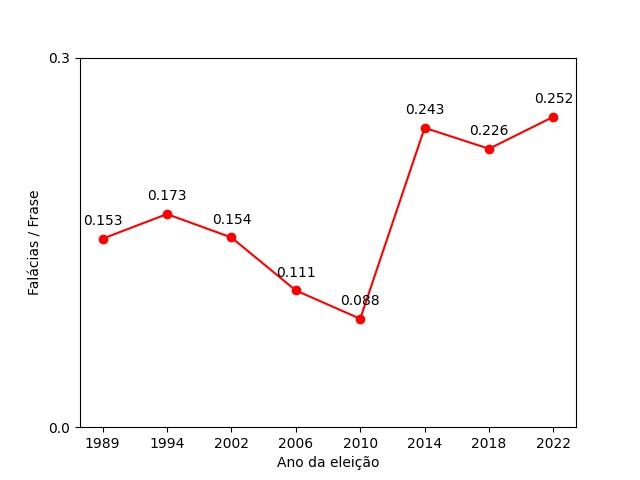
\includegraphics[scale=0.6]{media.png}
\end{center}

Este ensaio revela como a inovação nas redes sociais impactou significativamente a qualidade dos debates políticos no Brasil, introduzindo desafios éticos e sociais. A proliferação de tecnologias como fact-checking e gravações, embora úteis, não foi suficiente para conter o aumento de falácias e desinformação, particularmente em períodos eleitorais críticos.

Os resultados mostram uma correlação entre o uso de redes sociais e a polarização dos discursos políticos, que, por sua vez, influenciam negativamente a percepção pública e a qualidade do debate democrático. Portanto, é essencial que medidas sejam implementadas para promover uma maior responsabilidade no uso dessas plataformas e para educar o público sobre como discernir informações válidas de falácias.

A análise histórica dos debates presidenciais entre 1989 e 2022 destaca a necessidade de conscientização crítica sobre o uso de falácias nos discursos políticos. Somente assim será possível assegurar que o processo democrático se desenvolva em um ambiente mais transparente e informativo, contribuindo para escolhas mais conscientes por parte do eleitorado.

Em conclusão, a pesquisa sugere uma revisão das políticas de regulação de conteúdo nas redes sociais e um esforço conjunto entre educadores, mídia e plataformas tecnológicas para fomentar uma cultura de diálogo mais ética e informada.

A pesquisa evidencia como o uso de falácias em discursos políticos agrava a manipulação argumentativa. Além disso, ressalta o papel crucial das redes sociais na formação de bases ideológicas, facilitando a disseminação de falácias através dos novos meios de comunicação. A pesquisa também sublinha a maneira como esses dispositivos argumentativos contribuem para a construção de narrativas enganosas e manipulativas.


\bibliographystyle{sbc}
\bibliography{sbc-template}
\end{document}
